\documentclass{article}
\usepackage[a4paper, total={7in, 10in}]{geometry}
\usepackage{graphicx}
\usepackage{fontspec}
\usepackage{booktabs}
\usepackage{xltabular}
\usepackage[utf8]{inputenc}
\usepackage{hyperref}

\hypersetup{
    colorlinks=true,
    linkcolor=blue,
    filecolor=magenta,
    urlcolor=blue,
    pdftitle={Tesis de Carlos Santos Toro Vera}
}

%\setmainfont{Arial}
\graphicspath{ {./res/} }

\begin{document}

% vi:ft=tex
\begin{titlepage}
    \begin{center}
        \vspace*{1cm}
        \Large
        \textbf{PONTIFICIA UNIVERSIDAD CATOLICA DEL PERÚ}

        \vspace{0.5cm}
        \textbf{FACULTAD DE CIENCIAS E INGENIERÍA}

        \vspace{0.5cm}
        
\includegraphics[scale=0.8]{pucp}

        \vspace{1.5cm}
        \textbf{Desarrollo de un sistema web para la gestión de contenidos de información turística.}

        \normalsize
        \vspace{3.5cm}
        \textbf{Tesis Para optar por el Título de Ingeniero Informático que presenta el bachiller:}

        \Large
        \vspace{1.5cm}
        \textbf{Carlos Santos Toro Vera}

        \vspace{0.3cm}
        \textbf{20171878}

        \vspace{3cm}
        \textbf{Asesora: Doctora Mariuxi Alexandra Bruzza Moncayo}

        \textbf{Co-asesor: Doctor Manuel Francisco Tupia Anticona}

        \normalsize
        \vspace{3cm}
        {Lima, Marzo de 2023}
    \end{center}
\end{titlepage}



\section{Área}
Sistemas de información

\section{Asesores}
\begin{itemize}
    \item{Doctora Mariuxi Alexandra Bruzza Moncayo}
    \item{Doctor Manuel Francisco Tupia Anticona}
\end{itemize}

\section{Plan de trabajo}

Se llego a un acuerdo entre el tesista y los asesores. En este acuerdo se decidió
que se tendrían reuniones uno a uno de una hora los miércoles utilizando la
plataforma zoom, siendo esta reunión grabada para futura referencia.
Adicionalmente, toda comunicación adicional debe ser mediante el uso de correo electrónico.

Todo documento que se desee que los asesores lo revisen, tendrá que ser subido
a la plataforma de Google Drive configurado previo al inicio del curso. Finalmente,
el url del archivo subido sera adjuntado al correo electrónico que se enviara a
los asesores.

% vi:ft=tex

\newcolumntype{L}[1]{>{\hsize=#1\hsize\raggedright\arraybackslash}X}%
\newcolumntype{R}[1]{>{\hsize=#1\hsize\raggedleft\arraybackslash}X}%
\newcolumntype{C}[1]{>{\hsize=#1\hsize\centering\arraybackslash}X}%

\begin{xltabular}{\textwidth}{C{0.5} C{2.5} C{0.5} C{0.5}}
    \caption{Cronograma de reuniones}\label{tab:long} \\
    \toprule
    Semana & Tema & Fecha & Horario \\
    \midrule
    1 & Revisión de entregable EP1.1 con asesores. & 22/03/2023 & 16:00--17:00 \\
    \midrule
    1 & Avance de entregable EP1.1, levantamiento de observaciones y envio de avance a asesores. & 23/03/2023 & 20:00--22:00 \\
    \midrule


    1 & Avance de entregable EP1.2 y levantamiento de observaciones. & 25/03/2023 & 18:00--22:00 \\
    \midrule
    1 & Avance de entregable EP1.2 y levantamiento de observaciones. & 26/03/2023 & 18:00--22:00 \\
    \midrule
    2 & Avance de entregable EP1.2, levantamiento de observaciones y envio de avance a asesores. & 27/03/2023 & 20:00--22:00 \\
    \midrule
    2 & Avance de entregable EP1.2, levantamiento de observaciones y envio de avance a asesores. & 28/03/2023 & 20:00--22:00 \\
    \midrule
    2 & Revisión de entregable EP1.2 con asesores. & 29/03/2023 & 16:00--17:00 \\
    \midrule
    2 & Avance de entregable EP1.2, levantamiento de observaciones y envio de avance. & 30/03/2023 & 20:00--22:00 \\
    \midrule


    2 & Avance de entregable EP1.3 y levantamiento de observaciones. & 01/04/2023 & 18:00--22:00 \\
    \midrule
    3 & Avance de entregable EP1.3 y levantamiento de observaciones. & 02/04/2023 & 18:00--22:00 \\
    \midrule
    3 & Avance de entregable EP1.3, levantamiento de observaciones y envio de avance a asesores. & 03/04/2023 & 20:00--22:00 \\
    \midrule
    3 & Avance de entregable EP1.3, levantamiento de observaciones y envio de avance a asesores. & 04/04/2023 & 20:00--22:00 \\
    \midrule
    3 & Revisión de entregable EP1.3 con asesores. & 05/04/2023 & 16:00--17:00 \\
    \midrule
    3 & Avance de entregable EP1.3, levantamiento de observaciones y envio de avance. & 06/04/2023 & 20:00--22:00 \\
    \midrule


    3 & Avance de entregable EP1.4 y levantamiento de observaciones. & 08/04/2023 & 18:00--22:00 \\
    \midrule
    4 & Avance de entregable EP1.4 y levantamiento de observaciones. & 09/04/2023 & 18:00--22:00 \\
    \midrule
    4 & Avance de entregable EP1.4, levantamiento de observaciones y envio de avance a asesores. & 10/04/2023 & 20:00--22:00 \\
    \midrule
    4 & Avance de entregable EP1.4, levantamiento de observaciones y envio de avance a asesores. & 11/04/2023 & 20:00--22:00 \\
    \midrule
    4 & Revisión de entregable EP1.4 con asesores. & 12/04/2023 & 16:00--17:00 \\
    \midrule
    4 & Avance de entregable EP1.4, levantamiento de observaciones y envio de avance. & 13/04/2023 & 20:00--22:00 \\
    \midrule


    4 & Avance de entregable EP1.5 y levantamiento de observaciones. & 15/04/2023 & 18:00--22:00 \\
    \midrule
    5 & Avance de entregable EP1.5 y levantamiento de observaciones. & 16/04/2023 & 18:00--22:00 \\
    \midrule
    5 & Avance de entregable EP1.5, levantamiento de observaciones y envio de avance a asesores. & 17/04/2023 & 20:00--22:00 \\
    \midrule
    5 & Avance de entregable EP1.5, levantamiento de observaciones y envio de avance a asesores. & 18/04/2023 & 20:00--22:00 \\
    \midrule
    5 & Revisión de entregable EP1.5 con asesores. & 19/04/2023 & 16:00--17:00 \\
    \midrule
    5 & Avance de entregable EP1.5, levantamiento de observaciones y envio de avance. & 20/04/2023 & 20:00--22:00 \\
    \midrule


    5 & Avance de entregable E1 y levantamiento de observaciones. & 22/04/2023 & 18:00--22:00 \\
    \midrule
    6 & Avance de entregable E1 y levantamiento de observaciones. & 23/04/2023 & 18:00--22:00 \\
    \midrule
    6 & Avance de entregable E1, levantamiento de observaciones y envio de avance a asesores. & 24/04/2023 & 20:00--22:00 \\
    \midrule
    6 & Avance de entregable E1, levantamiento de observaciones y envio de avance a asesores. & 25/04/2023 & 20:00--22:00 \\
    \midrule
    6 & Revisión de entregable E1 con asesores. & 26/04/2023 & 16:00--17:00 \\
    \midrule
    6 & Avance de entregable E2.1, levantamiento de observaciones y envio de avance. & 27/04/2023 & 20:00--22:00 \\
    \midrule


    6 & Avance de entregable EP2.1 y levantamiento de observaciones. & 29/04/2023 & 18:00--22:00 \\
    \midrule
    7 & Avance de entregable EP2.1 y levantamiento de observaciones. & 30/04/2023 & 18:00--22:00 \\
    \midrule
    7 & Avance de entregable EP2.1, levantamiento de observaciones y envio de avance a asesores. & 01/05/2023 & 20:00--22:00 \\
    \midrule
    7 & Avance de entregable EP2.1, levantamiento de observaciones y envio de avance a asesores. & 02/05/2023 & 20:00--22:00 \\
    \midrule
    7 & Revisión de entregable EP2.1 con asesores. & 03/05/2023 & 16:00--17:00 \\
    \midrule
    7 & Avance de entregable EP2.1, levantamiento de observaciones y envio de avance. & 04/05/2023 & 20:00--22:00 \\
    \midrule


    7 & Avance de entregable E2 y levantamiento de observaciones. & 06/05/2023 & 18:00--22:00 \\
    \midrule
    8 & Avance de entregable E2 y levantamiento de observaciones. & 07/05/2023 & 18:00--22:00 \\
    \midrule
    8 & Avance de entregable E2, levantamiento de observaciones y envio de avance a asesores. & 08/05/2023 & 20:00--22:00 \\
    \midrule
    8 & Avance de entregable E2, levantamiento de observaciones y envio de avance a asesores. & 09/05/2023 & 20:00--22:00 \\
    \midrule
    8 & Revisión de avance para E2 con asesores. & 10/05/2023 & 16:00--17:00 \\
    \midrule
    8 & Avance de entregable E2, levantamiento de observaciones y envio de avance. & 11/05/2023 & 20:00--22:00 \\
    \midrule


    9 & No hay reunion & --- & --- \\
    \midrule


    9 & Avance de entregable E2 y levantamiento de observaciones. & 20/05/2023 & 18:00--22:00 \\
    \midrule
    10 & Avance de entregable E2 y levantamiento de observaciones. & 21/05/2023 & 18:00--22:00 \\
    \midrule
    10 & Avance de entregable E2, levantamiento de observaciones y envio de avance a asesores. & 22/05/2023 & 20:00--22:00 \\
    \midrule
    10 & Avance de entregable E2, levantamiento de observaciones y envio de avance a asesores. & 23/05/2023 & 20:00--22:00 \\
    \midrule
    10 & Revisión de entregable E2 con asesores. & 24/05/2023 & 16:00--17:00 \\
    \midrule
    10 & Avance de entregable E3, levantamiento de observaciones y envio de avance. & 25/04/2023 & 20:00--22:00 \\
    \midrule


    10 & Avance de entregable E3 y levantamiento de observaciones. & 27/05/2023 & 18:00--22:00 \\
    \midrule
    11 & Avance de entregable E3 y levantamiento de observaciones. & 28/05/2023 & 18:00--22:00 \\
    \midrule
    11 & Avance de entregable E3, levantamiento de observaciones y envio de avance a asesores. & 29/05/2023 & 20:00--22:00 \\
    \midrule
    11 & Avance de entregable E3, levantamiento de observaciones y envio de avance a asesores. & 30/05/2023 & 20:00--22:00 \\
    \midrule
    11 & Revisión de avance para E3 con asesores. & 31/05/2023 & 16:00--17:00 \\
    \midrule
    11 & Avance de entregable E3, levantamiento de observaciones y envio de avance. & 01/06/2023 & 20:00--22:00 \\
    \midrule


    11 & Avance de entregable E3 y levantamiento de observaciones. & 03/06/2023 & 18:00--22:00 \\
    \midrule
    12 & Avance de entregable E3, levantamiento de observaciones y envio de avance. & 04/06/2023 & 18:00--22:00 \\
    \midrule
    12 & Avance de entregable E4, levantamiento de observaciones y envio de avance a asesores. & 05/06/2023 & 20:00--22:00 \\
    \midrule
    12 & Avance de entregable E4, levantamiento de observaciones y envio de avance a asesores. & 06/06/2023 & 20:00--22:00 \\
    \midrule
    12 & Revisión de entregable E4 con asesores. & 07/06/2023 & 16:00--17:00 \\
    \midrule
    12 & Avance de entregable E4, levantamiento de observaciones y envio de avance. & 08/06/2023 & 20:00--22:00 \\
    \midrule


    12 & Avance de entregable E4 y levantamiento de observaciones. & 10/06/2023 & 18:00--22:00 \\
    \midrule
    13 & Avance de entregable E4 y levantamiento de observaciones. & 11/06/2023 & 18:00--22:00 \\
    \midrule
    13 & Avance de entregable E4, levantamiento de observaciones y envio de avance a asesores. & 12/06/2023 & 20:00--22:00 \\
    \midrule
    13 & Avance de entregable E4, levantamiento de observaciones y envio de avance a asesores. & 13/06/2023 & 20:00--22:00 \\
    \midrule
    13 & Revisión de entregable E4 con asesores. & 14/06/2023 & 16:00--17:00 \\
    \midrule
    13 & Avance de entregable E4, levantamiento de observaciones y envio de avance. & 15/06/2023 & 20:00--22:00 \\

    \bottomrule
\end{xltabular}



\newpage

\section{Descripción}

El proyecto consiste en desarrollar un sistema web que permita gestionar
información turística a nivel de un país, tomando como referencia la web:
\url{https://www.visitportugal.com/es}.\\
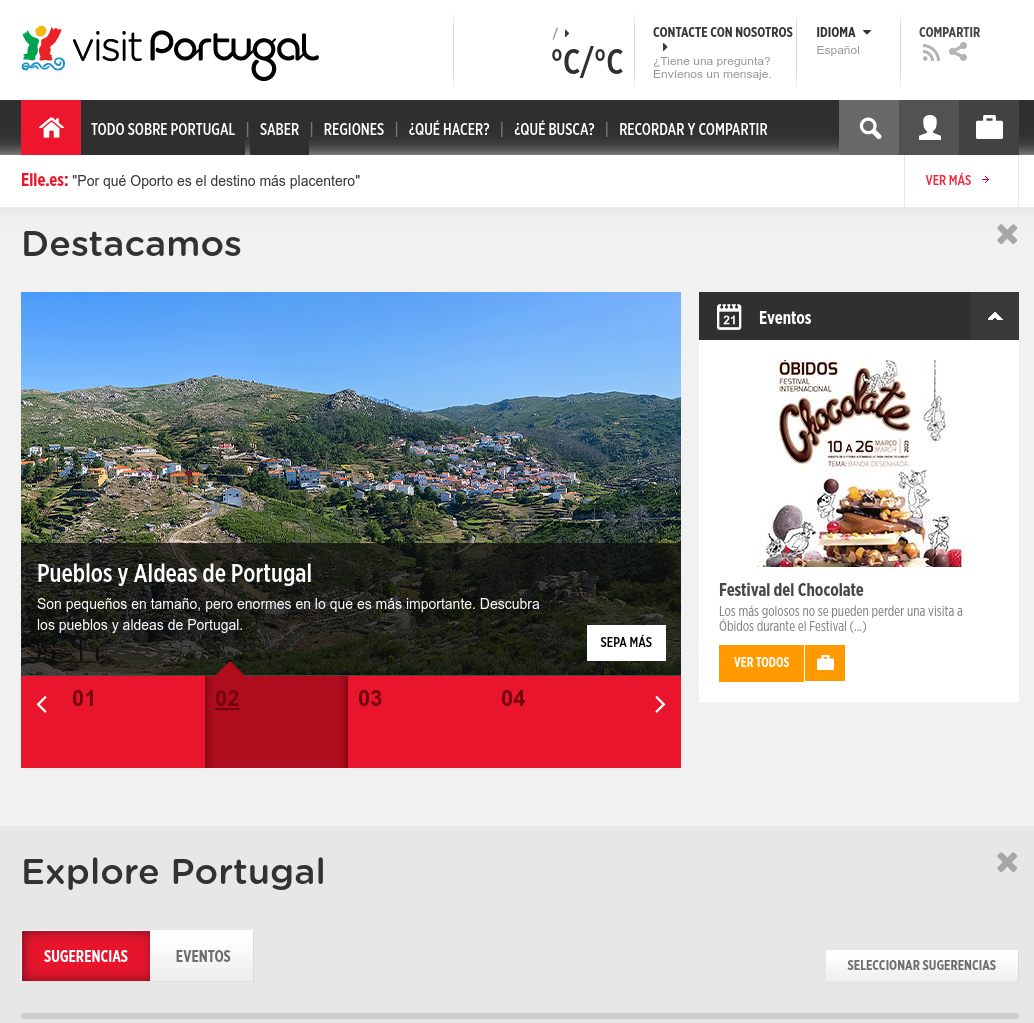
\includegraphics[width=\textwidth,height=\textheight,keepaspectratio]{visit-portugal-site.png}
Es verdad que la mayoría de instituciones gubernamentales en el mundo y empresas
turísticas locales ya poseen información para turistas, pero esta información
tiende a ser poco interactiva o no existente en los casos en que la empresa turística
no posee convenios con empresas locales en las ubicaciones que un turista este interesado.\\
Esta tesis propone una solución de software la cual remediara los problemas
anteriormente mencionados, además de incluir funcionalidades adicionales tales como,
pero sin limitarse a:
\begin{itemize}
    \item{Mostrar información básica para el ingreso al país.}
    \item{Mostrar mapas y folletos del lugar.}
    \item{Mostrar posibles actividades para cada tipo de usuario.}
    \item{Mostrar enlaces de interés.}
    \item{Mostrar historia del lugar y noticias actuales.}
    \item{Buscador de actividades, eventos, alojamiento, transporte.}
    \item{Mostrar imágenes y videos de posible interés al usuario.}
    \item{Planificación de viajes (generación de paquetes personalizados).}
\end{itemize}
Gran parte de la información requerida se obtendrá utilizando fuentes públicas
de cada gobierno local. Esta información será ingresada utilizando un sistema
simple de administración de contenido incluido en el sistema. Esta información
se mostrara a los usuarios utilizando una aplicación web la cual tendrá funcionalidades
adicionales las cuales le permitan trabajar en dispositivos táctiles y `All-in-one'.
Adicionalmente, se implementara un algoritmo propietario el cual se encargara
de la generación de paquetes de viajes. La generación de estos paquetes turísticos
evitaría que los turistas tengan que utilizar múltiples paginas web para planear
su viajes ya que esta solución de software tendría toda la información centralizada.\\
La generación de los paquetes depende de condiciones iniciales. Estas condiciones
iniciales incluirían el lugar inicial del viaje, lugar destino y además de un
itinerario de actividades que los turistas deseen realizar. Luego que el usuario
ha definido estas condiciones iniciales, se utilizara el algoritmo mencionado
anteriormente para generar información la cual incluiría instrucciones para llegar
al lugar de destino, las empresas que realizan esos viajes, los horarios que
tienen disponibles y los costos promedios del viaje. Si es que los turistas desean
comer algo, se mostrara información de los restaurantes cercanos al lugar junto con
el costo promedio de las comidas que ofrecen. Finalmente, de acuerdo al itinerario
de actividades que el turista ha elegido, se mostrara información acerca de los
negocios que proveen tales experiencias junto con información adicional para que
el turista se comunique con estos.

\end{document}
